% ----------------------------------------------
\begin{figure}[htbp]
  \centering
  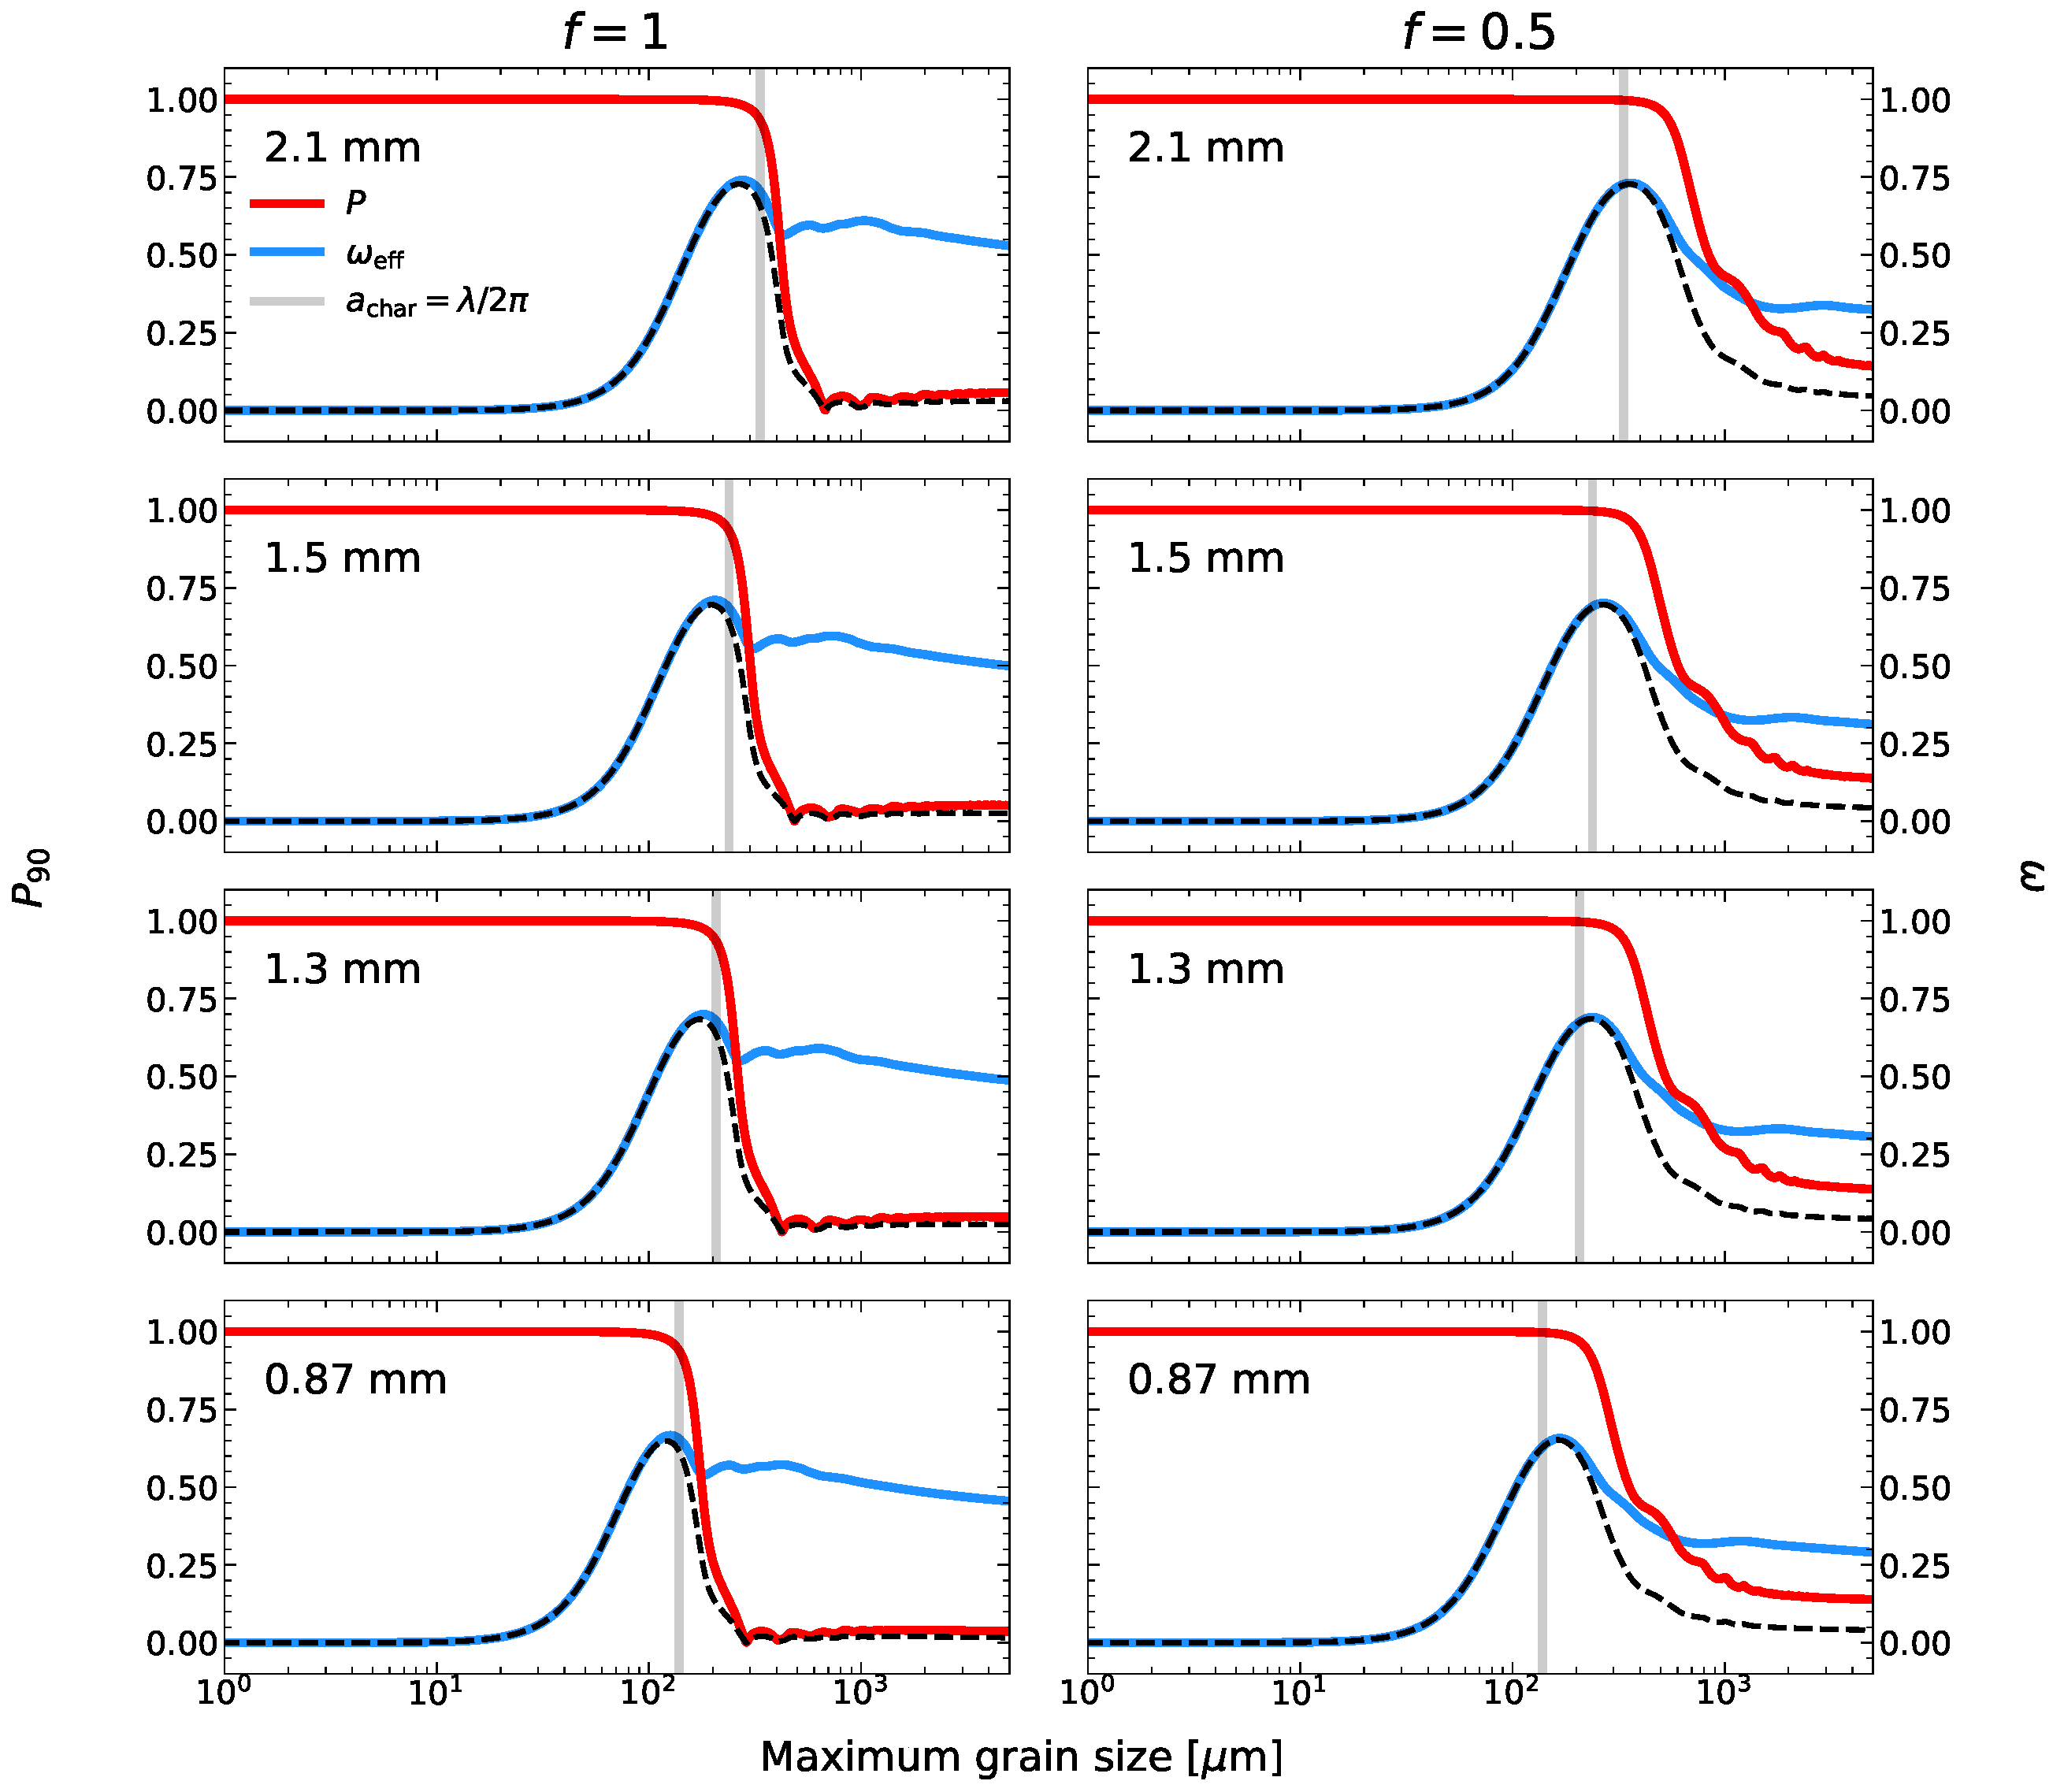
\includegraphics[width=0.99\textwidth]{WRITEUP_AND_IMAGES/IMAGES/WRITEUP/DustModels/P_vs_w_vs_grainsize_grid_smooth_porosities.pdf}
  \caption{Same as Figure \ref{fig: Kataoka2015Figure3Recreation} but for \Pw not \PweffNS.}
  \label{fig: Kataoka2015Figure3Recreation_Pw}
\end{figure}
% ----------------------------------------------


% ------------------------------------------------------
\begin{table}[h!]
\centering
\caption{Same as Table \ref{tab: amax_peak_values} but for \Pw and not \PweffNS. \add{references to plots} \intextref{add}}
%\label{tab:amax_peak_values}
\begin{tabular}{lcccc}
\toprule
\textbf{Grain Size ($\boldsymbol{\mu}$m)} & \textbf{\bfour} & \textbf{\bfive} & \textbf{\bsix} & \textbf{\bseven} \\
\midrule

$a_{\text{char}}$
& 334.23
& 238.73
& 206.90
& 138.46 \\

$a_{\max}$ (spherical)
& 266.02
& 196.46
& 173.46
& 120.70 \\


$a_{\max}$ (irregular)
& 333.19 
& 240.77 
& 213.26 
& 147.62 \\



\bottomrule
\end{tabular}
%\label{tab: amax_peak_values_Pw}
\end{table}
% ------------------------------------------------------



\subsection{\Pw and compact}
% ----------------------------------------------
\begin{figure}[htbp]
  \centering

  \begin{minipage}[t]{0.48\textwidth}
    \centering
    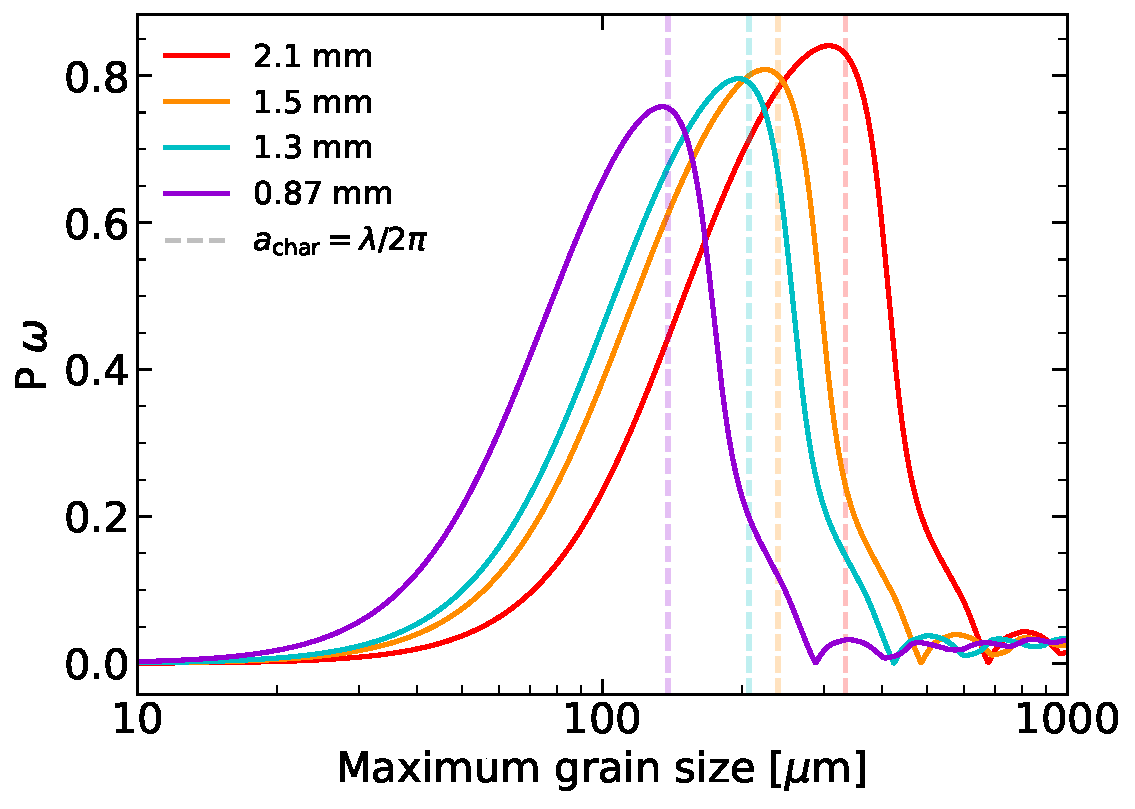
\includegraphics[width=\textwidth]{WRITEUP_AND_IMAGES/IMAGES/WRITEUP/DustModels/Pw_vs_grainsize_smooth.pdf}
  \end{minipage}
  \hfill
  \begin{minipage}[t]{0.48\textwidth}
    \centering
    
\includegraphics[width=\textwidth]{WRITEUP_AND_IMAGES/IMAGES/WRITEUP/DustModels/glitterin/Pw_vs_grainsize.pdf}
  \end{minipage}

  \caption{Same as Figure \ref{fig: Pweff_vs_grainsize} but for \Pw and not \PweffNS.}
  \label{fig: Pw_vs_grainsize_appendix}
\end{figure}
% ----------------------------------------------




% ------------------------------------------------------
\begin{table}[h!]
\centering
\caption{Same as Table \ref{tab: dust_model_fits_irregular} but for fits using $\omega$ and not \weffNS. \refintext{add}}
\begin{tabular}{lccc}
\toprule
\textbf{Fit Case} &  \textbf{Scale Factor (SF)} & $\boldsymbol{\chi_\mathcal{P}^2}$ & \textbf{$\boldsymbol{\amaxEQ}$ ($\boldsymbol{\mu}$m)} \\
\midrule

All wavelengths  & \textbf{1.77} & \textbf{4.58} & \textbf{212} \\
No \bfive               & 1.81 & 6.16 & 214 \\
Just \bfour and \bseven & 1.83 & 8.41 & 215 \\
\bottomrule
\end{tabular}
\label{tab: dust_model_fits_irregular_no_eff}
\end{table}
% ------------------------------------------------------




% ----------------------------------------------------------------
\begin{figure}[htbp]
  \centering
  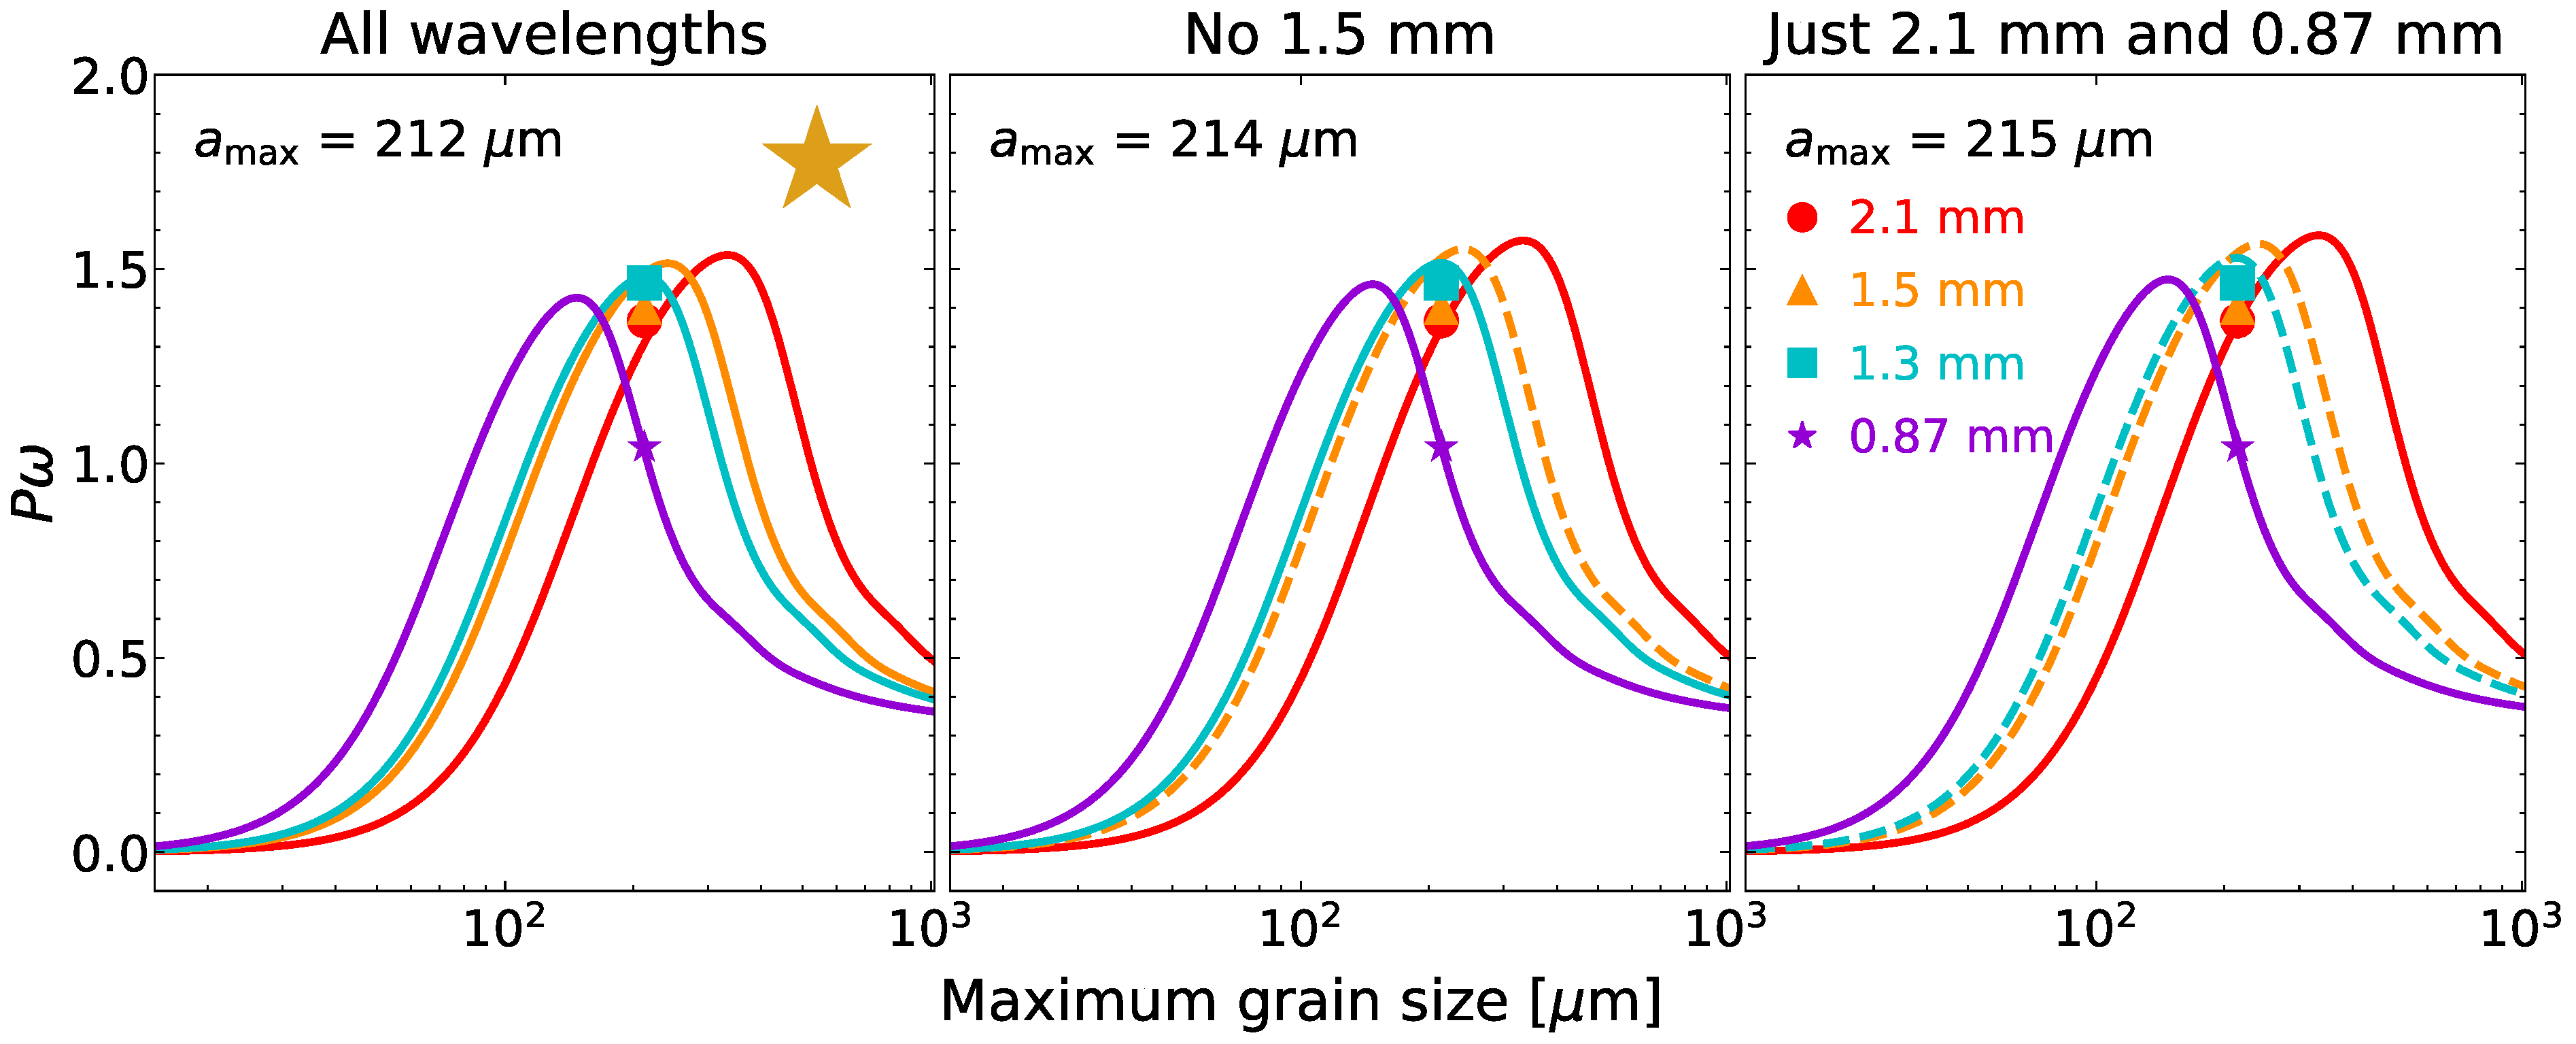
\includegraphics[width=0.99\textwidth]{WRITEUP_AND_IMAGES/IMAGES/WRITEUP/glitterin/DustModelPlot_GlitterinGrid_only3.pdf}
  \caption{Same as Figure \ref{fig: irregular_fits} but for \Pw and not \PweffNS. \code{Change to $P$ not P, wrong panel has star} \refintext{add}} 
  \label{fig: irregular_fits_w}
\end{figure}
% ----------------------------------------------------------------


